\documentclass[journal]{IEEEtran}
%\usepackage[left=2.2cm,right=2.2cm,top=2.5cm,bottom=2.5cm]{geometry}
\usepackage[utf8]{inputenc}
\usepackage[english]{babel}
\usepackage{minted}
\usepackage{booktabs}
\usepackage{commath}
\usepackage{float}
\usepackage{mathtools}
\usepackage{color}
\usepackage{amsthm}
\usepackage{parskip}
\usepackage{graphicx}
\usepackage{epstopdf}

\theoremstyle{definition}
\newtheorem{defn}{Definition}[section]


\usepackage[binary-units=true]{siunitx}

\newcommand{\py}[1]{\mintinline{python}{#1}}
\newcommand{\java}[1]{\mintinline{java}{#1}}
\newcommand{\sql}[1]{\mintinline{sql}{#1}}

\usepackage{hyperref}

\title{Architecture and Performance of Computer Systems \\ Project on Client-Server Application Performance}
\author{Gilles Peiffer (24321600), Liliya Semerikova (64811600)}
\date{January 6, 2020}

\begin{document}

\maketitle

\begin{abstract}
	This paper studies the performance of a client-server application (more specifically, a MariaDB server and a remote computer sending randomized SQL queries to that server) in order to first measure the effect of various parameters (such as the query type or the rate at which queries are sent) on the response time of the application, and second, to compare these results to the expected values using the various models of queuing theory.
\end{abstract}

\section*{Introduction}
The answers to the various tasks are given in Sections~\ref{sec:task1} and \ref{sec:task2}.
Section~\ref{sec:char} describes how to reproduce the experiments we did.

\section{Task 1: Measurements}
\label{sec:task1}
For the first task, we first study the average query response time (and the influence of various parameters on it), then we try to find out what factors influence the response time, and where potential bottlenecks lie.

\subsection{Characteristics for Reproducibility}
\label{sec:char}
All experiments were done on two different physical computers:
\begin{itemize}
	\item The server was MariaDB 10.4.11 running on an Early 2015 MacBook Pro with Ubuntu 18.04 LTS ``Bionic Beaver'', with \SI{8}{\giga\byte} of \SI{1867}{\mega\hertz} of DDR3 RAM memory, a \SI{2.9}{\giga\hertz} Intel Core i5 CPU, an Intel Iris Graphics 6100 \SI{1536}{\mega\byte} GPU and \SI{500}{\giga\byte} of Flash storage.
	\item The remote client was running on a 2016 MacBook Pro with macOS Catalina 10.15.2, with \SI{8}{\giga\byte} of \SI{2133}{\mega\hertz} of LPDDR3 RAM memory, a \SI{2.9}{\giga\hertz} Dual-Core Intel Core i5 CPU, an Intel Iris Graphics 550 \SI{1536}{\mega\byte} GPU and \SI{251}{\giga\byte} of Flash storage.
\end{itemize}

The tests were done on various networks:
\begin{itemize}
	\item a WiFi network in one of the team members' student residence, and
	\item the home network of the other team member, on which the final tests were done (the ones appearing on plots).
\end{itemize}
This network has a download and upload speeds on the order of \SI{2}{\mega\bit\per\second} according to the \href{https://fast.com/en/gb}{\url{FAST.com}} speed test.

For the measurements, no significant warmup was needed, as no amount of queries showed any signs of instability beyong what one would expect on a real-world physical network.
All tests were repeated multiple times, and under different network loads, while final results were obtained when there was no other activity on the network.

Every query is made using a new connection, on a different thread.
For this purpose, we defined a new Java class, \java{SQLThread}, which extends the \java{Thread} class, queries the database when its \java{run()} method is called.
The server is configured to allow up to three concurrent threads, by using the \mintinline[breaklines]{bash}{sudo mysqld --user mysql --innodb-thread-concurrency=3} command.

The measurements were written into a csv file by the Java code, which was then read by a short Python script which generates the plots using \py{pandas} and \py{seaborn}.

\subsection{Average Query Response Time}
\begin{defn}[Response time]
	The \emph{response time} is typically treated as the elapsed time from the moment that a user enters a command or activates a function until the time that the application indicates that the command or function has completed.
\end{defn}

The following section studies the influence of the query type and the query rate on the response time of the application.

\subsubsection{Influence of the Query Type}
For this experiment, various types of queries were considered, based on the ones provided in the client template:
\begin{itemize}
	\item ``\java{GetAverage}'' queries compute the average salary over a certain subset of rows of the table, where the number of rows and the starting row are randomly determined\footnote{In order to simplify the modeling task of Section~\ref{sec:task2}, this random value is generated in a way that the number of rows over which the query operates is exponentially distributed.} outside of the timed section and are passed to the server using the \sql{LIMIT} and \sql{OFFSET} keywords.
	\item ``\java{Select}'' queries select a subset of rows (randomly, according to the same rules as for the previous query) and returns the result.
	\item ``\java{Write}'' queries insert a row into the database.
\end{itemize}

For every type, tests were run multiple times, in order to get an idea of the average response time without inter-arrival pauses.
For the actual tests, every thread waits a certain amount of time before starting its execution.
This amount is a exponentially-distributed random variable, in order to mimic a Poisson process, where the parameter \(\lambda\) is different for every type of query and depends on the average response time as well as the number of concurrent threads allowed on the MariaDB server.
In order to single out the influence of the query type, this value was chosen so as to make it very improbable that queries would have to wait before being answered.

The result is shown on Figure~\ref{fig:query_influence}.
\begin{figure}[!hbtp]
	\centering
	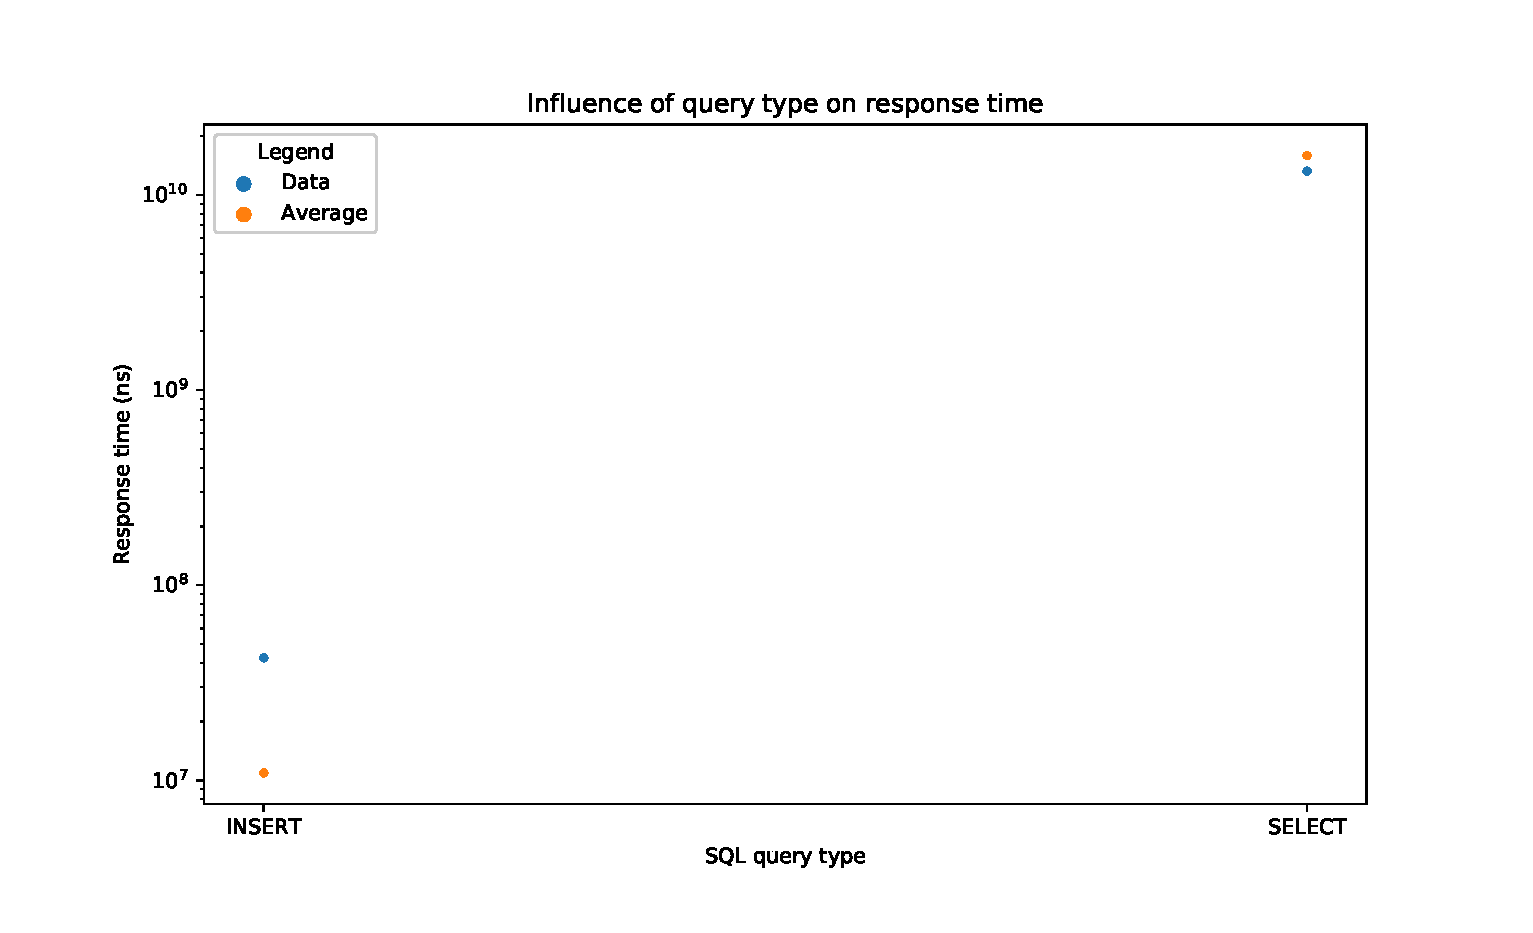
\includegraphics[width=\columnwidth]{../plotting/query_influence}
	\caption{Influence of query type on response time}
	\label{fig:query_influence}
\end{figure}
The \(y\)-axis is shown with logarithmic units in order to clearly show the difference in response time for the various queries.
The \java{Write} query is on average the fastest, which is logical since it only needs to insert a single row into the database; the \java{Select} and \java{GetAverage} queries are separated because the \sql{LIMIT} values are very different for both requests, with \java{Select} queries having a much higher value than the others.

Using the command line tools \mintinline{bash}{top} and \mintinline{bash}{nethogs}, we saw that the \mintinline{bash}{mysql} process only took up about \SI{2}{\percent} of the total available RAM, whereas CPU usage was usually around \SI{10}{\percent} though it was slightly higher for the \sql{SELECT}-based queries than for the \sql{INSERT}-based ones.

\subsubsection{Influence of the Number of Queries Per Second}
Next, in order to control the influence of the rate at which queries are sent, we force queries to all be of the same type (\java{GetAverage}), and play around with the sleep delay before each thread sends its query.

We still use the same kind of delay as in the previous section, that is, one with exponential inter-arrival times.
By changing the parameter of the distribution in order to shorten or lengthen the expected waiting time between queries, we were able to observe the influence of the rate on the average response time.

The results of this experiment are shown in Figure~\ref{fig:rate_influence}.
\begin{figure}[!hbtp]
	\centering
	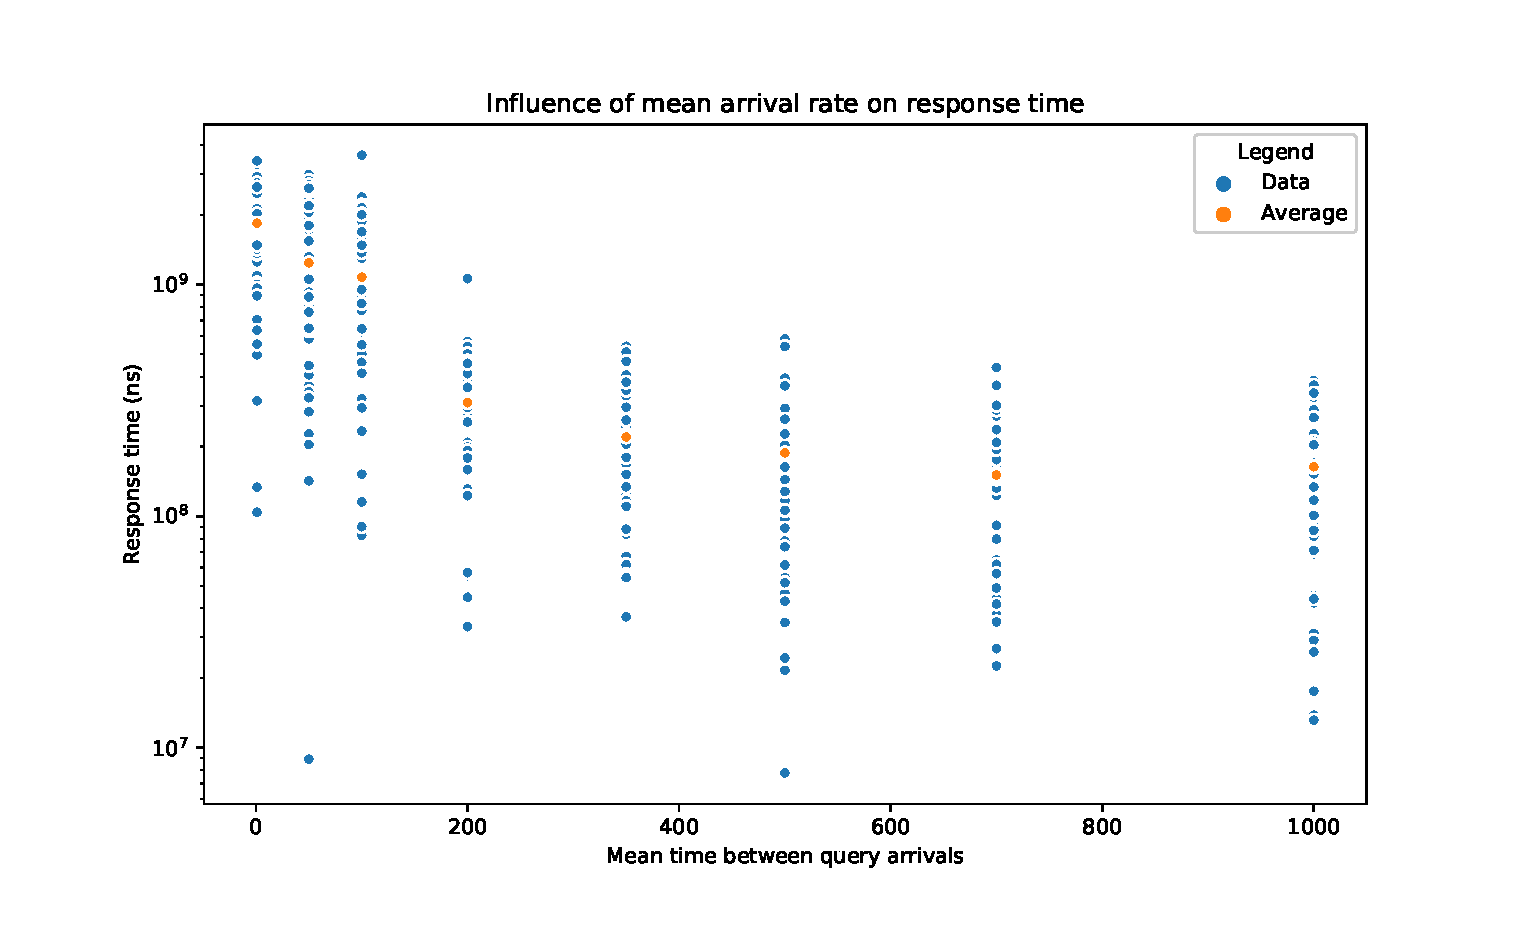
\includegraphics[width=\columnwidth]{../plotting/rate_influence}
	\caption{Influence of request rate on response time}
	\label{fig:rate_influence}
\end{figure}

\textcolor{red}{TODO}

\subsection{Factors Influencing the Query Response Time and Possible Bottlenecks}
We have already noted in the previous sections that the query type and the rate at which queries are sent have an influence on the response time.
In this section, we will give some other factors influencing the response time, and identify where bottlenecks lie.

\textcolor{red}{TODO}

\section{Task 2: Modeling}
\label{sec:task2}
\subsection{Queuing Station Model}
Using the theoretical results described in the lecture notes, we now attempt to model the client-server application using one of the models from queuing theory covered in class.

\subsubsection{Determining the Parameters}
\textcolor{red}{TODO}

\subsection{Comparison to the Real Data}
\textcolor{red}{TODO}

\section*{Conclusion}
 
\end{document}
